% \documentclass{article}
% \usepackage{hyperref, graphics}
% \begin{document}
\title{Git Assignment Week 4 }
\maketitle
\section{Introduction:}

I am Minhajul Alam Rahat, a second-year PhD student at the UCCS CS department. My research focus is on embedded system security. Specifically, I am interested in device firmware vulnerability analysis. I am an enthusiast of technology and knowledge. I like practical problem-solving and innovation. I want to contribute to society through my research work in the future. I look forward to working in academia to continue my research work in the future and, at the same time, help students become good researchers.
I look forward to learning research methodologies in a more systematic approach while doing the CS 6000 course. I believe that it will help me broaden my thinking while trying to devise a plan or methodology to solve a problem. This course will also help me read research papers efficiently and hone my skills in using different tools for my research work. I have already met several creative and skilled research people in the class, and I am excited to share our ideas and passions for research. I hope to understand how other people in the research community are doing research in their respective fields. 

\begin{figure}[h]
    \centering
    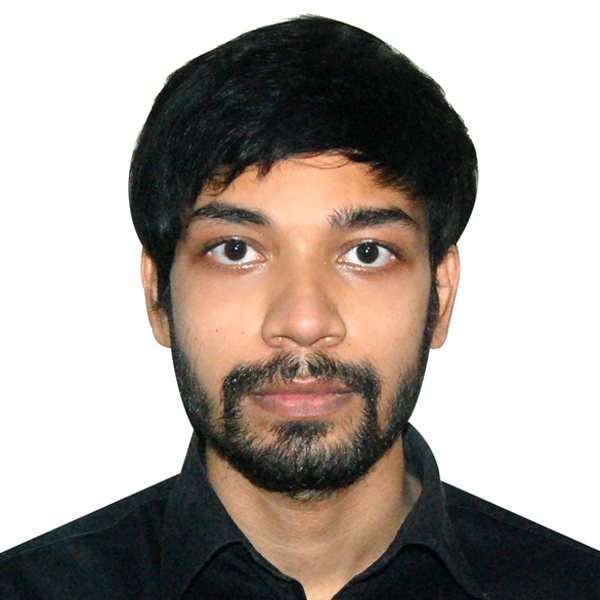
\includegraphics{minhajul.jpg}
    \caption{My Photo ID}
    \label{fig:personalPic}
\end{figure}

\section{Related Code:}

I am working in firmware binary analysis techniques. One of the work related to my topic is Firmalice. Firmalice is a binary firmware analysis framework. It is based on a symbolic execution engine which can find authentication bypass flaws in embedded device firmware. Link to the code for this framwork: 

\url{https://github.com/angr/pyvex}

\section{Questions:}
\subsection{01: What are the limitations of achieving this goal as you need sufficient data and also bytecode analysis is sometimes hard?}

The hard part of analyzing firmware binary is we may not know which compiler was used during compilation (stripped binaries) or the  internal structure of the code (symbol tables, entry point) etc.  
\subsection {02: For the binary analysi, do you plan to look at supply chain compromise attacks?}
% \end{document}
